\documentclass{article}
\usepackage[spanish,thai,thainumber]{babel}
\usepackage[utf8x]{inputenc}
\usepackage{fonts-tlwg}
\usepackage{graphicx}
\usepackage{wrapfig}
\usepackage{multicol}
\usepackage{blindtext}
\usepackage{wallpaper}
\usepackage{mdframed}
\usepackage{titlesec}
\usepackage{titling}

%\usepackage[top=2cm, bottom=2cm, outer=0cm, inner=0cm]{geometry}
\graphicspath{ {./images/} }

%\newfontfamily\Calluna{Calluna-Regular.otf}
\begin{document}
\title{ตัวอย่างการใช้ UTF-8}
\author{writeLaTeX}
\begin{titlepage}
    \centering
    \vspace*{2cm}
    \Huge
    \ThisLRCornerWallPaper{1.0}{masia2.png}
    Pannagiri
    \emph{El monestir l'Aragall}
    \vfill
    \Large
    \vspace{0.8cm}
\end{titlepage}
\maketitle
%\ThisLRCornerWallPaper{1.0}{masia2.png}
\section{ภาษาที่ทดสอบ}

ภาษาไทย -- \foreignlanguage{english}{English}

\section{ใช้คำสั่งเปลี่ยนภาษา}

ภาษาไทย -- \selectlanguage{english} English \selectlanguage{thai}

\section{ใช้ environment}

ภาษาไทย ภาษาไทย ภาษาไทย ภาษาไทย ภาษาไทย ภาษาไทย ภาษาไทย ภาษาไทย ภาษาไทย ภาษาไทย 
ภาษาไทย ภาษาไทย ภาษาไทย ภาษาไทย ภาษาไทย ภาษาไทย ภาษาไทย ภาษาไทย ภาษาไทย ภาษาไทย 
ภาษาไทย ภาษาไทย ภาษาไทย ภาษาไทย ภาษาไทย ภาษาไทย ภาษาไทย ภาษาไทย ภาษาไทย ภาษาไทย 
ภาษาไทย ภาษาไทย ภาษาไทย ภาษาไทย ภาษาไทย ภาษาไทย ภาษาไทย ภาษาไทย ภาษาไทย ภาษาไทย 

Pannagiri es el monasterio de los nagas, un lugar sagrado en la tradición budista.
\begin{wrapfigure}{r}{0.25\textwidth} %this figure will be at the right
    \centering
    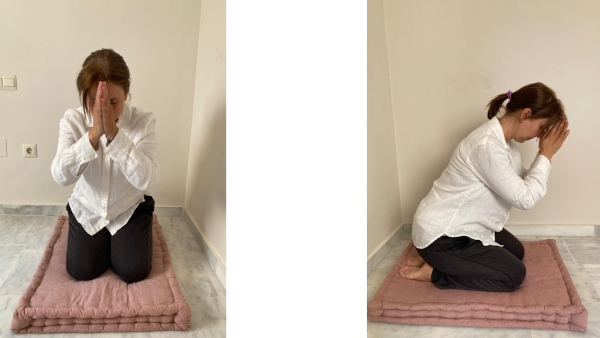
\includegraphics[width=0.25\textwidth]{vandami_woman.jpg}
\end{wrapfigure}
On the other side, if you are only interested on
certain values yhgfgdou can use the contour plot, you 
can use the contour plot, you can use the contour 
plot, you can use the contour plot, you can use 
the contour plot, you can use the contour plot, 
you can use the contour plot, like the one on the left.

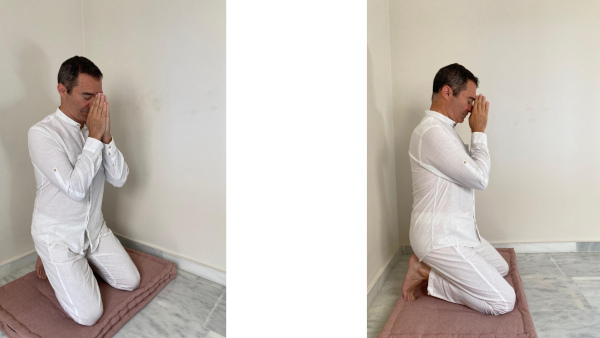
\includegraphics[width=5cm, height=4cm]{vandami_man.jpg}

On the other side, if you are only interested on 
certain values you can use the contour plot, you 
can use the contour plot, you can use the contour 
plot, you can use the contour plot, you can use the 
contour plot, you can use the contour plot, 
you can use the contour plot, 
like the one on the left.

\begin{wrapfigure}{r}{0.25\textwidth} %this figure will be at the right
    \centering
    \includegraphics[width=0.25\textwidth]{wave.png}
\end{wrapfigure}

\foreignlanguage{thai}{\Blindtext}




\begin{multicols*}{2}
[
\section{First Section}
All human things are subject to decay. And when fate summons, Monarchs must obey.
]
\Blindtext
\end{multicols*}

\begin{multicols}{2}
[
\section{Nuestra Tradicion}
All human things are subject to decay. And when fate summons, Monarchs must obey.
]
Hello, here is some text without a meaning.  This text should show what 
a printed text will look like at this place.
\begin{wrapfigure}{l}{0.7\linewidth}
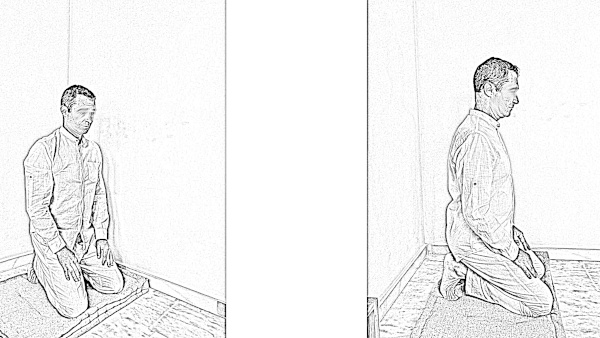
\includegraphics[width=\linewidth]{prep-man-ai.jpg}
\caption{This is the Overleaf logo}
\end{wrapfigure}
If you read this text, you will get no information.  Really?  Is there 
no information?  Is there.
\foreignlanguage{english}{\blindtext
\vfill


}

\columnbreak
\foreignlanguage{thai}{ขอให้คำขวัญแก่โยมทั้งหลาย และลูกศิษย์ใหม่ที่เดินทางจากลอนดอน มาพักอยู่ที่วัดหนองป่าพง ขอให้ทำความเข้าใจในธรรมะที่ได้ศึกษาแล้วที่วัดหนองป่าพงนี้โดยย่อก็คือ ให้ปฏิบัติให้พ้นทุกข์ในวัฏฏสงสาร

ขอให้โยมจำไว้ในใจว่า อารมณ์ทั้งหลายนั้น จะเป็นอารมณ์ที่พอใจก็ตาม หรืออารมณ์ที่ไม่พอใจก็ตามอารมณ์ทั้งสองอย่างนี้ มันเหมือนงูเห่า งูเห่ามันมีพิษมากถ้ามันฉกคนแล้วก็ทำให้ถึงแก่ความตายได้ อารมณ์นี้ก็เหมือนกับงูเห่าที่มีพิษร้ายนั้น อารมณ์ที่พอใจก็มีพิษมากอารมณ์ที่ไม่พอใจก็มีพิษมาก มันทำให้จิตใจของเราไม่เป็นเสรี ทำให้จิตใจไขว้เขว จากหลักธรรมของพระพุทธเจ้า

วันนี้จึงขอให้โอวาทย่อๆแก่โยม ขอให้เป็นผู้มีสติอยู่ทั้งกลางวันกลางคืน จะยืน จะเดิน จะนั่ง จะนอนก็ให้นอนด้วยสติ นั่งด้วยสติ เดินด้วยสติ ยืนด้วยสติ จะพูดก็พูดด้วยสติ จะทำอะไรๆก็ให้มีสติอยู่ด้วยทั้งนั้น

เมื่อมีสติแล้ว สัมปชัญญะความรู้ตัวมันก็จะเกิดขึ้นมา สติกับสัมปชัญญะเป็นของคู่กัน เมื่อทั้งสองอย่างนี้เกิดขึ้นพร้อมกันแล้ว ก็จะนำปัญญาให้เกิดตามทีนี้เมื่อมีทั้งสติ สัมปชัญญะปัญญาแล้ว ก็จะเป็นผู้ที่ตื่นอยู่ ทั้งกลางวันและกลางคืน

ธรรมะที่พระพุทธเจ้าท่านทรงสอนนั้น ไม่ใช่ธรรมะที่เพื่อฟังเฉยๆหรือรู้เฉยๆ แต่เป็นธรรมะที่ต้องปฏิบัติ ต้องทำให้เกิดขึ้น ต้องทำให้มีขึ้นในใจของเราให้ได้ จะไปที่ไหนก็ให้มีธรรมะ จะพูดก็ให้มีธรรมะ จะเดินก็ให้มีธรรมะ จะนอนก็ให้มีธรรมะ จะทำอะไรๆก็ให้มีธรรมะทั้งนั้น

คำว่า "มีธรรมะ" นี้ก็คือ จะทำอะไรก็ตาม จะพูดอะไรก็ตาม ให้ทำด้วยปัญญา ให้พูดด้วยปัญญา ให้นึกคิดด้วยปัญญา ผู้ใดมีสติ สัมปชัญญะ ควบกับปัญญาอยู่ตลอดเวลาแล้ว ผู้นั้นย่อมอยู่ใกล้พระพุทธเจ้าทุกเมื่อ

ดังนั้น แม้เมื่อโยมจากวัดหนองป่าพงนี้ไปแล้ว ก็จงเป็นผู้ปฏิบัติ ให้ธรรมะทั้งหลายมารวมอยู่ที่ใจ มองลงไปที่ใจ ให้เห็นสติ ให้เห็นสัมปชัญญะ ให้มีปัญญา เมื่อมีทั้งสามอย่างนี้แล้ว มันจะมีการปล่อยวาง รู้จักเกิดแล้วมันก็ดับ ดับแล้วมันก็เกิด เกิดแล้วมันก็ดับ

ที่เรียกว่า "เกิดๆ ดับๆ" นี้คืออะไร คืออารมณ์ซึ่งมันเกิดขึ้นแล้วมันก็ดับไป ดับแล้วมันก็เกิดขึ้นมา ในทางธรรมะเรียกว่าการเกิดดับ มันก็มีเท่านี้ ทุกข์มันเกิดขึ้นแล้ว ทุกข์มันก็ดับไป ทุกข์ดับไปแล้ว ทุกข์ก็เกิดขึ้นมา นอกเหนือจากนี้ไป ก็ไม่มีอะไรมีแต่ทุกข์เกิด แล้วทุกข์ก็ดับไป มีเท่านี้

เมื่อเห็นเช่นนี้แล้ว จิตของเราก็จะเห็นแต่การเกิด-ดับอยู่เสมอ เมื่อเห็นการเกิด-ดับอยู่เสมอ ทุกวันทุกเวลา ตลอดทั้งกลางวัน ตลอดทั้งกลางคืน ตลอดทั้งการยืน เดิน นั่ง นอน ก็จะเห็นได้ว่ามันไม่มีอะไรจริงๆมีแต่เกิด-ดับอยู่เท่านี้เอง แล้วทุกอย่างมันก็จบอยู่ตรงนี้ ย ภาษาไทย ภาษาไทย ภาษาไทย ภาษาไทย 
}

\end{multicols}

\end{document}